%\documentclass[xcolor={dvipsnames}]{beamer}

\documentclass[xcolor={dvipsnames}, notes]{beamer}

\usetheme{Warsaw}

\usepackage{inputenc}
\usepackage{amsmath}
\usepackage{amsthm}
\usepackage{graphicx}
%\usepackage{geometry}
\usepackage{tasks}
\ifodd\textwidth
  \addtolength{\textwidth}{1sp}
\fi

\setbeamertemplate{theorems}[numbered]


\newtheorem{prop}{Proposition}

\newcommand{\po}{\textcolor{BlueViolet}{po}}
\newcommand{\rf}{\textcolor{Green}{rf}}
\newcommand{\co}{\textcolor{BurntOrange}{co}}
\newcommand{\mo}{\textcolor{Red}{mo}}
\newcommand{\hb}{\textcolor{NavyBlue}{hb}}
\newcommand{\fr}{\textcolor{RubineRed}{fr}}
\newcommand{\xhb}{\textcolor{NavyBlue}{xhb}}
\newcommand{\rfe}{\textcolor{Green}{rfe}}
\newcommand{\rfi}{\textcolor{Green}{rfi}}
\newcommand{\sw}{\textcolor{BurntOrange}{sw}}
\newcommand{\jhb}{\textcolor{NavyBlue}{jhb}}
\newcommand{\jmo}{\textcolor{Red}{jmo}}
\newcommand{\eco}{\textcolor{WildStrawberry}{eco}}


\title{Explaining Relaxed Memory Models with Program Transformations}
\subtitle{Ori Lahav and Viktor Vafeiadis}

\author{Presented by \\ Akshay Gopalakrishnan}

\begin{document}
    
    \begin{frame}

        \maketitle

    \end{frame}

    \begin{frame}{Introduction}
    
        \begin{itemize}
            \item Uniprocessor semantics respects sequential consistency.
            \item Mutliprocessor has more behaviors that programs can exhibit.
            \item They are either justified by hardware features such as Load/Store buffers, speculation, etc.
            \item Or they can be justified by the program begin optimized in various passes by a compiler. 
            \item Semantics of such behaviors however, are not specified using such intuition, rather, per-execution or event-structure based axiomatic models, or more non-trivial operational models.
            \item This paper investigates upto what extent such memory consistency models can be specified using program transformations.  
        \end{itemize}
        
    \end{frame}

    \begin{frame}{Contributions}

        \begin{itemize}
            \item TSO can be explained by W-R reordering and Read-after-Write elimination over SC.
            \item RA cannot be specified in the same manner - counter example to show this.
            \item A substantial subset of POWER can be specified in a similar way over a stronger model of power - SPOWER
            \item ARM however, cannot be done the same way.
            \item Advantage of using this to simplify compilation correctness proofs.
        \end{itemize}
        
    \end{frame}

    \begin{frame}{Axiomatic Model Definitions}

        Axiomatic events:
        \begin{itemize}
            \item Read event $\Re = Ld \cup U$.
            \item Write event $W = St \cup U$. 
            \item Fence - Can be of various types depending on the architecture / language's memory model.
        \end{itemize}

        Binary relations:
        \begin{itemize}
            \item {\po} - Program order per thread.
            \item {\rf} - Between a read and the write from which its read value comes.
            \item {\co} - Order between writes/updates to same location.
            \item {\mo} - Order between memory writes/updates.
        \end{itemize}

    \end{frame}

    \begin{frame}{Sequential Consistency (SC)}
        
        Additional binary relations:
        \begin{itemize}
            \item {\hb} - Happens before $ \hb = (\po \cup \rf)^{+} $
            \item {\fr} - Reads before (from reads) $ \fr = (\rf^{-1};\mo_{|loc}) $ 
        \end{itemize}

        SC is defined using the following irreflexivity relations that must hold for any program execution:
        \begin{tasks}(2)
            \task {\mo} total order on W/U.
            \task {\hb} irreflexive.
            \task {\mo;\hb} irreflexive.
            \task {\fr;\hb} irreflexive.
            \task {\fr;\mo} irreflexive.
            \task {\fr;\mo;\hb} irreflexive.
        \end{tasks}

    \end{frame}

    \begin{frame}{Figures to explain above axioms of irreflexivity}
        
        \begin{figure}
            \makebox[\textwidth][c]{
                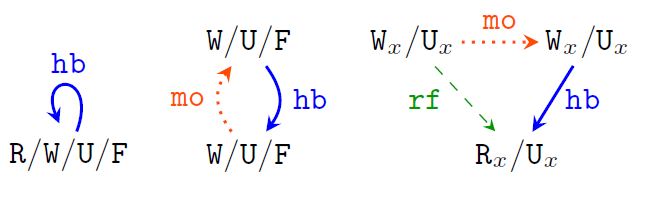
\includegraphics[scale=0.5]{SC-Def1.PNG}
            }
        \end{figure}

        \begin{figure}
            \makebox[\textwidth][c]{
                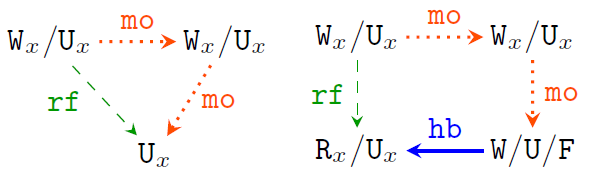
\includegraphics[scale=0.5]{SC-Def2.PNG}
            }
        \end{figure}

    \end{frame}

    \begin{frame}{Total Store Order (TSO)}

        Additional binary relations:
        \begin{itemize}
            \item {\xhb} - Happens before $ \xhb = (\po \cup \rf)^{+} $
            \item {\fr} - Reads before (from reads) $ \fr = (\rf^{-1};\mo_{|loc}) $ 
            \item {\rfe} - Reads from external $\rf \text{ \textbackslash} \ \po$
        \end{itemize}

        x86 TSO is defined using the following irreflexivity relations that must hold for any program execution:
        \begin{tasks}(2)
            \task {\mo} is a strict total order on W/U/F.
            \task {\xhb} irreflexive.
            \task {\mo;\xhb} irreflexive.
            \task {\fr;\xhb} irreflexive.
            \task {\fr;\mo} irreflexive.
            \task {\fr;\mo;\rfe;\po} irreflexive.
            \task {\fr;\mo;$[U \cup F]$;\po} irreflexive.
        \end{tasks}

    \end{frame}

    \begin{frame}{Figures to explain the last two axioms of irreflexivity.}
            
        \begin{figure}
            \makebox[\textwidth][c]{
                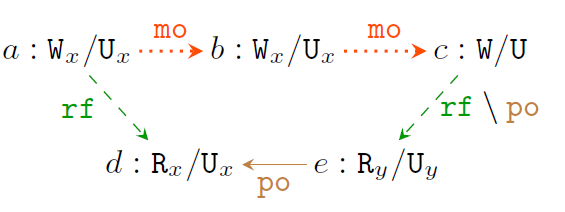
\includegraphics[scale=0.5]{TSO-Def1.PNG}
            }
        \end{figure}

        \begin{figure}
            \makebox[\textwidth][c]{
                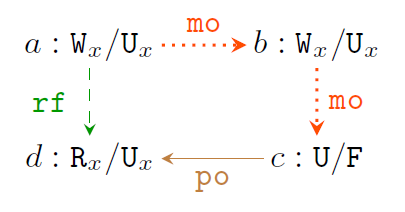
\includegraphics[scale=0.5]{TSO-Def2.PNG}
            }
        \end{figure}

    \end{frame}

    \begin{frame}{TSO Equivalence}

        TSO is precisely categorized by write-read reordering and read-after-write elimination over SC. 
        \begin{theorem}
            A plain execution G is TSO-consistent iff $G \longmapsto^{*}_{TSO} G'$ for some SC-consistent execution $G'$.
        \end{theorem}
        where $\longmapsto^{*}_{TSO}$ implies we either do write-read reordering or read-after-write elimination.
    
    \end{frame}

    \begin{frame}{Proof elements}

        \begin{prop}
            If $G \longmapsto^{*}_{TSO} G'$ and $G'$ is TSO consistent, then so is $G$.
        \end{prop}

        \begin{prop}
            If $G$ is TSO-consistent execution, then so is $RemoveWR(G,a,b)$.
        \end{prop}

        \begin{prop}
            If $G$ is TSO-consistent execution, then so is $ReorderWR(G,a,b)$ if $\langle a,b \rangle \notin \mo;\rf$.
        \end{prop}

    \end{frame}

    \begin{frame}{Proof elements cntd}
        \begin{prop}
            Suppose $G$ is TSO-consistent but not SC-consistent, then $G \longmapsto^{*}_{TSO} G'$ for some TSO-consistent execution $G'$.   
        \end{prop}
    \end{frame}

    \begin{frame}{Release Acquire (RA)}

        This model exhibits non-multi-copy-atomicity, meaning, threads may observe updates/writes in different orders.
        Here {\mo} is defined only between events W/U accessing the same memory.
        The axioms then are as follows:
        \begin{tasks}(2)
            \task {\mo} disjoint union of relations $\mo_{x}$ each of which are strict total orders. 
            \task {\hb} irreflexive.
            \task {\mo;\hb} irreflexive.
            \task {\fr;\hb} irreflexive.
            \task {\fr;\mo} irreflexive.
        \end{tasks}
        where {\hb}, {\fr} are as that of Sequential consistency.

    \end{frame}

    \begin{frame}{Why RA cannot be described the same way}

        %Insert IRIW example here to show cannot be described by SC/TSO
        \begin{figure}
            \makebox[\textwidth][c]{
                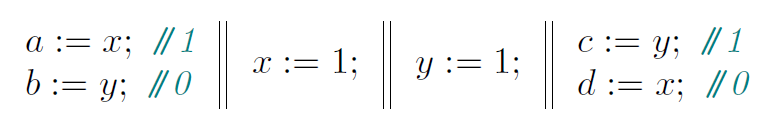
\includegraphics[scale=0.6]{IRIW_RA.PNG}
            }
        \end{figure}

        %Insert IRIW example here to show how sequentialization works 
        \begin{figure}
            \makebox[\textwidth][c]{
                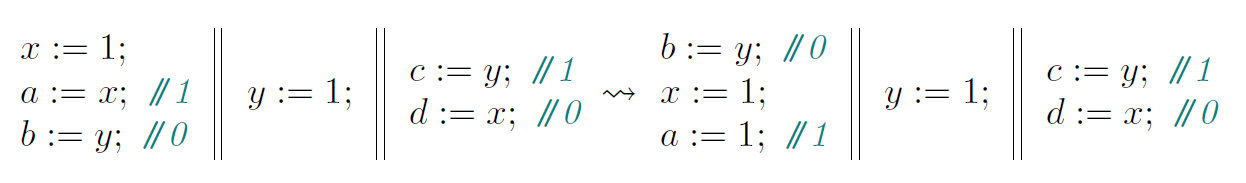
\includegraphics[scale=0.5]{IRIW_SEQ.PNG}
            }
        \end{figure}

    \end{frame}

    \begin{frame}{Why RA cannot be described the same way}
        
        %Insert example showing no sound transformation of RA can explain the behavior
        \begin{figure}
            \makebox[\textwidth][c]{
                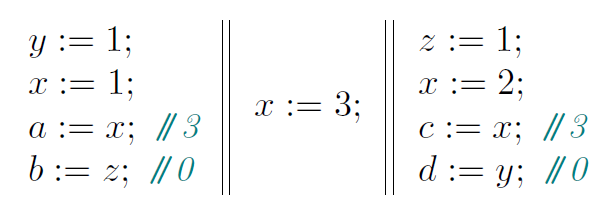
\includegraphics[scale=0.6]{NOTRANSF_RA.PNG}
            }
        \end{figure}

    \end{frame}

    \begin{frame}{Similar Analysis for POWER and ARMv7/v8}
        
        \begin{itemize}
            \item POWER can be specified using SPOWER, whose only difference is it disallows $\po \cup \rf$ cycles.
            \item Then POWER is equivalent to reordering over SPOWER (you keep reordering until only dependency order = program order).
            \item ARM cannot be specified in a similar way (perhaps refer to figure in notes section that cannot be explained by program transformations)
        \end{itemize}
        
    \end{frame}

    \begin{frame}{Advantage of Transformational Models: Compiler Correctness}

        Consider $[[P]]_{M}$ to be behaviors of program $P$ under memory model $M$. 
        Assume we have a compilation scheme from source $C$ to target $A$ (code gen phase: direct mapping of instructions).
        Let $M_{C}$ and $M_{A}$ be their respective memory models.
        Then compiler correctness requires: 
        \begin{align*}
            \forall P_{C}.[[compile(P_{C})]]_{M_{A}} \ \subseteq \ [[P_{C}]]_{M_{C}}. 
        \end{align*}  

    \end{frame}

    \begin{frame}{Compiler Correctness simplified using results in paper}

        Theorem 1 and 2 provide us with the following property:
        \begin{align*}
            \forall P_{C}.[[compile(P_{C})]]_{M_{A}} \ 
                \subseteq \ 
            \cup \{[[P'_{A}]]_{SM_{A}} | P'_{A}. compile(P_{C}) \longmapsto^{*}_{M_{A}} P'_{A} \}.  
        \end{align*}  
        where $SM_{A}$ is the stronger memory model than $M_{A}$ (like SC for TSO in Theorem 1).

    \end{frame}

    \begin{frame}{Simplified proof requirements}

        Using above info, compiler correctness boils down to two conditions. 
        \begin{itemize}
            \item Compilation should be correct for the strong model $SM_{A}$.
            \item There should be a set of source program transformations sound for source model $M_{C}$ and it should capture all target transformations from a compiled program. 
        \end{itemize}

    \end{frame}

    \begin{frame}{Thank you}

        Questions ?

    \end{frame}

\end{document}